\documentclass[12pt]{article}

\usepackage[margin=1in]{geometry}
\usepackage{amsmath,amssymb}
\usepackage{graphicx}
\usepackage{booktabs}
\usepackage{natbib}
\usepackage{setspace}
\usepackage{hyperref}
\usepackage{caption}
\usepackage{subcaption}
\usepackage{float}
\usepackage{pdflscape}
\usepackage[T1]{fontenc}
\usepackage{lmodern}
\usepackage{catchfile}
\newcommand{\inputifexists}[1]{\IfFileExists{#1}{\input{#1}}{\textit{[Table not yet generated.]}}}

\bibliographystyle{aer}

\onehalfspacing

\title{Urban Air Pollution and Time Losses: \\
Evidence from Cyclists in London --- Revisited}

\author{Joris Klingen \and Jos van Ommeren}

\date{\today}

\begin{document}

\maketitle

\begin{abstract}
We replicate and extend \citet{klingen2020urban}, who found that a 10~ppb increase in ozone reduces cycling speed by 0.3--0.4\% using 42 million London bike-share trips (2013--2017). Extending the sample to 112 million trips through 2025, we find a negative ozone--speed relationship in all four identification strategies. The within-day estimate is stable across periods, at about 0.05~km/h per 10~ppb. The within-cyclist estimate, based on pseudo-cyclists defined within a calendar year-month, is about half the original estimate and smaller after 2017, but remains statistically significant.

\medskip
\noindent \textit{Keywords}: air pollution, ozone, physical effort, cycling, productivity, replication \\
\noindent \textit{JEL Codes}: I18, J24, Q53, R41
\end{abstract}

\newpage

%% ============================================================
\section{Introduction} \label{sec:intro}
%% ============================================================

\citet{klingen2020urban} provided novel evidence that ambient ozone reduces cycling speed, using 42 million Santander Cycles trips during 2013--2017. Their preferred within-day estimate implied that a 10~ppb increase in ozone reduces speed by about 0.4\%, with effects emerging at concentrations as low as 20~ppb---far below regulatory standards.

We revisit their analysis with two objectives. First, we replicate the original results on the 2013--2017 sample, implementing the same four identification strategies (within-day, between-day, spatio-temporal, cyclist panel) without traffic controls, which the original study showed to be inconsequential. Second, we extend the analysis to 2013--2025, with 112 million trips. We also estimate models on the post-2017 subsample alone (2018--2025) to test whether the relationship holds in a period that includes COVID-19, the Ultra Low Emission Zone expansion, and substantial cycling infrastructure changes.

Our replication confirms the core findings. The within-day ozone coefficient is similar in the replication, extended and post-2017 samples. The between-day and spatio-temporal strategies yield negative coefficients, although the spatio-temporal estimate is imprecise for 2013--2017. The cyclist-panel estimate is smaller than in the original study, which we attribute to a stricter definition of pseudo-cyclists.\footnote{The original study pooled the same calendar month over years, so that a pseudo-cyclist could combine trips made several years apart.} Robustness checks---non-linearity analysis, lag/lead tests, and median speed regressions---support the original conclusions.


%% ============================================================
\section{Methods and Data} \label{sec:methods}
%% ============================================================

We implement the four identification strategies of \citet{klingen2020urban}; see their paper for details. All models are estimated on weekdays only.

\paragraph{Within-day.} Hourly city-level speed is regressed on ozone (per 10~ppb), flexible weather controls (temperature dummies, pressure, humidity, rain, radiation dummies, wind, 8-hour temperature and rain lags), and co-pollutant controls (SO$_2$, NO$_x$ and PM$_{2.5}$ dummies), with day and day-of-week$\times$hour fixed effects. WLS with trip counts as weights; SEs clustered by date.

\paragraph{Between-day.} Daily aggregates with year-month and day-of-week fixed effects.

\paragraph{Spatio-temporal.} Zone-day aggregates (5 monitoring zones, 2~km radius; a trip is assigned to a zone if both its origin and destination station are within 2~km of the monitor), with day, zone, and zone-month (or zone-week) fixed effects and NO$_x$ dummies.

\paragraph{Cyclist panel.} Pseudo-cyclists are identified from repeat trips on the same route (origin and destination station), in the same clock hour and the same calendar year-month, with at most one trip per day, at least 4 trips, and departure-time regularity below the 5th percentile of the random uniform distribution. Unlike the original study, which pooled the same calendar month over all years, a pseudo-cyclist is confined to one year-month. A check on New York's Citi Bike, where trips of members in 2017--2019 report the rider's birth year and gender, suggests that this makes pseudo-cyclists considerably purer: within a pseudo-cyclist, 88\% of trip pairs share birth year and gender, against 80\% when the calendar month is pooled over years (2\% for two random members). Electric bikes, introduced in September 2022 and about 2~km/h faster than classic bikes for the same pseudo-cyclist, are excluded. Cyclist fixed effects absorb route and time-of-day preferences.

\paragraph{Data.} Trip data are from Transport for London's Santander Cycles. TfL reports clock times in GMT until mid-September 2013 and in UK local time thereafter; we convert all times to GMT to match the air quality and weather data. Air quality data (O$_3$, NO$_2$, NO, PM$_{2.5}$, SO$_2$) are from the London Air Quality Network (5 stations). Weather data are from the Open-Meteo archive. The replication sample covers 2013--2017 ($\approx$41M trips), the extended sample 2013--2025 ($\approx$112M trips), and the post-2017 sample 2018--2025 ($\approx$70M trips).

Table~\ref{tab:desc} reports descriptive statistics. Mean ozone is higher in the post-2017 period (25.2 vs.\ 18.7~ppb) while NO$_x$ has declined substantially (21.8 vs.\ 44.6~ppb), consistent with ULEZ effects. Mean cycling speed is slightly higher in recent years (12.5 vs.\ 12.0~km/h).

\begin{table}[H]
\centering
\caption{Descriptive statistics (hourly, trip-weighted).}
\label{tab:desc}

\medskip
\small Panel A: Replication (2013--2017).

\begin{tabular}{lrrrr}
\toprule
Statistic & Mean & St Dev. & Min & Max \\
\midrule
Speed (km/h) & 11.98 & 1.67 & 5.85 & 17.75 \\
Distance (km) & 2.82 & 0.29 & 1.40 & 5.36 \\
Duration (sec) & 1110.40 & 325.03 & 443.33 & 10658.68 \\
Number of trips & 1821.43 & 1082.04 & 4.00 & 6893.00 \\
Ozone (O\textsubscript{3}, ppb) & 18.69 & 11.65 & 0.04 & 78.28 \\
Nitrogen oxides (NO\textsubscript{x}, ppb) & 44.60 & 33.83 & 1.38 & 509.24 \\
Particulate matter (PM\textsubscript{2.5}, $\mu$g/m\textsuperscript{3}) & 13.23 & 10.17 & -2.60 & 114.87 \\
Sulphur dioxide (SO\textsubscript{2}, ppb) & 1.05 & 0.88 & -0.29 & 92.72 \\
\bottomrule
\end{tabular}


\medskip
\small Panel B: Post-2017 (2018--2025).

\begin{tabular}{lrrrr}
\toprule
Statistic & Mean & St Dev. & Min & Max \\
\midrule
Speed (km/h) & 12.47 & 1.65 & 1.24 & 22.72 \\
Distance (km) & 3.06 & 0.33 & 0.96 & 11.56 \\
Duration (sec) & 1118.89 & 299.41 & 247.42 & 24468.88 \\
Number of trips & 1865.29 & 1057.95 & 1.00 & 6642.00 \\
Ozone (O\textsubscript{3}, ppb) & 25.22 & 12.75 & 0.07 & 99.77 \\
Nitrogen oxides (NO\textsubscript{x}, ppb) & 21.85 & 18.87 & 0.28 & 270.19 \\
Particulate matter (PM\textsubscript{2.5}, $\mu$g/m\textsuperscript{3}) & 8.88 & 7.33 & -2.65 & 151.62 \\
Sulphur dioxide (SO\textsubscript{2}, ppb) & 0.59 & 0.63 & -0.69 & 52.24 \\
\bottomrule
\end{tabular}


\medskip
\footnotesize Means and standard deviations weighted by number of trips per hour.
\end{table}


%% ============================================================
\section{Results} \label{sec:results}
%% ============================================================

\subsection{Within-day estimation}

Table~\ref{tab:within} presents the within-day results. In the replication sample, a 10~ppb increase in ozone reduces speed by 0.047~km/h (column~1), close to the original estimate of $-0.053$. The effect is similar in the full extended sample ($-0.057$, column~2) and the post-2017 subsample ($-0.050$, column~3), all significant at the 1\% level.

The sorting tests show small effects of ozone on trip distance (columns~4--6) and log trips (columns~7--9). In the extended and post-2017 samples, a 10~ppb increase reduces mean distance by about 0.009~km (0.3\%) and raises the number of trips by 0.2--0.3\%. These effects are too small to suggest that the speed effect is driven by compositional changes.

\begin{table}[H]
\centering
\caption{Within-day estimation.}
\label{tab:within}
\begingroup
\centering
\begin{tabular}{lccccccccc}
   \tabularnewline \midrule \midrule
   Dependent Variables: & \multicolumn{3}{c}{mean\_speed} & \multicolumn{3}{c}{mean\_dist} & \multicolumn{3}{c}{log(n\_trips)}\\
                         & Speed (R)       & Speed (E)       & Speed (P)       & Dist (R) & Dist (E)        & Dist (P)        & Trips (R) & Trips (E)      & Trips (P) \\   
   Model:                & (1)             & (2)             & (3)             & (4)      & (5)             & (6)             & (7)       & (8)            & (9)\\  
   \midrule
   \emph{Variables}\\
   O3\_10                & -0.0706$^{***}$ & -0.0823$^{***}$ & -0.0719$^{***}$ & 0.0014   & -0.0130$^{***}$ & -0.0146$^{***}$ & -0.0001   & 0.0041$^{***}$ & 0.0041$^{***}$\\   
                         & (0.0147)        & (0.0103)        & (0.0119)        & (0.0035) & (0.0026)        & (0.0030)        & (0.0011)  & (0.0008)       & (0.0009)\\   
   \midrule
   \emph{Fixed-effects}\\
   date                  & Yes             & Yes             & Yes             & Yes      & Yes             & Yes             & Yes       & Yes            & Yes\\  
   dow\_hour\_daylight   & Yes             & Yes             & Yes             & Yes      & Yes             & Yes             & Yes       & Yes            & Yes\\  
   \midrule
   \emph{Fit statistics}\\
   Observations          & 31,092          & 78,974          & 47,882          & 31,092   & 78,974          & 47,882          & 31,092    & 78,974         & 47,882\\  
   R$^2$                 & 0.92575         & 0.92556         & 0.93499         & 0.92022  & 0.92296         & 0.92651         & 0.99843   & 0.99785        & 0.99814\\  
   Within R$^2$          & 0.21836         & 0.18148         & 0.21175         & 0.23067  & 0.18726         & 0.24359         & 0.98310   & 0.97724        & 0.97805\\  
   \midrule \midrule
   \multicolumn{10}{l}{\emph{Clustered (date) standard-errors in parentheses}}\\
   \multicolumn{10}{l}{\emph{Signif. Codes: ***: 0.01, **: 0.05, *: 0.1}}\\
\end{tabular}
\par\endgroup


\medskip
\footnotesize WLS with trip counts as weights. SEs clustered by date. (R) = 2013--2017, (E) = 2013--2025, (P) = 2018--2025.
\end{table}


\subsection{Between-day estimation}

Table~\ref{tab:between} reports between-day results. The replication coefficient ($-0.246$, column~1) is larger than the within-day estimate, consistent with the original study and with the fact that between-day variation in ozone may capture additional cumulative exposure effects. The post-2017 estimate ($-0.076$, column~3) is smaller but remains significant at the 5\% level. The distance and trip-count coefficients are small and mostly insignificant.

\begin{table}[H]
\centering
\caption{Between-day estimation.}
\label{tab:between}
\begingroup
\centering
\begin{tabular}{lccccccccc}
   \tabularnewline \midrule \midrule
   Dependent Variables: & \multicolumn{3}{c}{mean\_speed} & \multicolumn{3}{c}{mean\_dist} & \multicolumn{3}{c}{log(n\_trips)}\\
                & Speed (R)       & Speed (E)       & Speed (P)      & Dist (R)     & Dist (E) & Dist (P) & Trips (R)     & Trips (E) & Trips (P) \\   
   Model:       & (1)             & (2)             & (3)            & (4)          & (5)      & (6)      & (7)           & (8)       & (9)\\  
   \midrule
   \emph{Variables}\\
   O3\_10       & -0.2467$^{***}$ & -0.1120$^{***}$ & -0.0766$^{**}$ & 0.0113$^{*}$ & 0.0037   & 0.0004   & -0.0032$^{*}$ & -0.0010   & $-6\times 10^{-5}$\\    
                & (0.0540)        & (0.0272)        & (0.0324)       & (0.0060)     & (0.0033) & (0.0040) & (0.0018)      & (0.0010)  & (0.0012)\\   
   \midrule
   \emph{Fixed-effects}\\
   yearmonth    & Yes             & Yes             & Yes            & Yes          & Yes      & Yes      & Yes           & Yes       & Yes\\  
   dow          & Yes             & Yes             & Yes            & Yes          & Yes      & Yes      & Yes           & Yes       & Yes\\  
   \midrule
   \emph{Fit statistics}\\
   Observations & 1,302           & 3,349           & 2,047          & 1,302        & 3,349    & 2,047    & 1,302         & 3,349     & 2,047\\  
   R$^2$        & 0.53854         & 0.68191         & 0.73590        & 0.80743      & 0.90031  & 0.87641  & 0.99524       & 0.99508   & 0.99534\\  
   Within R$^2$ & 0.29476         & 0.20948         & 0.23013        & 0.56863      & 0.47900  & 0.45356  & 0.98748       & 0.98714   & 0.98800\\  
   \midrule \midrule
   \multicolumn{10}{l}{\emph{Clustered (date) standard-errors in parentheses}}\\
   \multicolumn{10}{l}{\emph{Signif. Codes: ***: 0.01, **: 0.05, *: 0.1}}\\
\end{tabular}
\par\endgroup


\medskip
\footnotesize WLS with daily trip counts as weights. SEs clustered by date. Fixed effects: year-month and day-of-week.
\end{table}


\subsection{Spatio-temporal estimation}

Table~\ref{tab:spatial} reports the spatio-temporal results. In the replication sample, the zone-month specification yields a near-zero coefficient (column~1), while the zone-week specification gives $-0.049$ (column~2), both imprecisely estimated---consistent with the wide confidence intervals in the original study. In the extended sample, the zone-week estimate is $-0.075$ and significant at the 1\% level (column~4). In the post-2017 sample, both specifications yield negative coefficients ($-0.047$ and $-0.089$), with the zone-week estimate significant at the 5\% level (column~6).

\begin{table}[H]
\centering
\caption{Spatio-temporal estimation (dependent variable: speed).}
\label{tab:spatial}
\begingroup
\centering
\begin{tabular}{lcccccc}
   \tabularnewline \midrule \midrule
   Dependent Variable: & \multicolumn{6}{c}{mean\_speed}\\
                & Speed-M(R) & Speed-W(R) & Speed-M(E) & Speed-W(E)      & Speed-M(P) & Speed-W(P) \\   
   Model:       & (1)        & (2)        & (3)        & (4)             & (5)        & (6)\\  
   \midrule
   \emph{Variables}\\
   O3\_10       & 0.0046     & -0.0397    & -0.0377    & -0.0752$^{***}$ & -0.0509    & -0.0916$^{**}$\\   
                & (0.0411)   & (0.0461)   & (0.0263)   & (0.0287)        & (0.0346)   & (0.0364)\\   
   \midrule
   \emph{Fixed-effects}\\
   date         & Yes        & Yes        & Yes        & Yes             & Yes        & Yes\\  
   zone         & Yes        & Yes        & Yes        & Yes             & Yes        & Yes\\  
   zone\_month  & Yes        &            & Yes        &                 & Yes        & \\  
   zone\_week   &            & Yes        &            & Yes             &            & Yes\\  
   \midrule
   \emph{Fit statistics}\\
   Observations & 5,893      & 5,875      & 14,354     & 14,315          & 8,461      & 8,440\\  
   R$^2$        & 0.95254    & 0.96949    & 0.95859    & 0.97361         & 0.96106    & 0.97531\\  
   Within R$^2$ & 0.02009    & 0.01644    & 0.00747    & 0.00880         & 0.00901    & 0.01278\\  
   \midrule \midrule
   \multicolumn{7}{l}{\emph{Clustered (date) standard-errors in parentheses}}\\
   \multicolumn{7}{l}{\emph{Signif. Codes: ***: 0.01, **: 0.05, *: 0.1}}\\
\end{tabular}
\par\endgroup


\medskip
\footnotesize WLS with zone-day trip counts as weights. SEs clustered by date. M = zone-month FE, W = zone-week FE.
\end{table}


\subsection{Cyclist panel estimation}

Table~\ref{tab:panel} presents the cyclist panel results across all three periods. The panel contains 836,027 pseudo-cyclists and 6.0 million trips. The replication coefficients ($-0.014$ and $-0.016$) are about half the original study's range of $-0.026$ to $-0.031$ (their Table~4), which plausibly reflects our stricter definition of pseudo-cyclists, confined to one year-month. The extension and post-2017 coefficients are smaller still ($-0.009$ and $-0.007$ for all distances), but remain statistically significant, so the within-cyclist ozone effect persists.

\begin{table}[H]
\centering
\caption{Cyclist panel estimation.}
\label{tab:panel}
\inputifexists{../output/tables/table4_panel_combined.tex}

\medskip
\footnotesize OLS with cyclist FE and day-of-week FE. SEs clustered by hour. Columns 1--2: replication (2013--2017), 3--4: extension (2013--2025), 5--6: post-2017 (2018--2025). Odd columns: all distances; even columns: trips $\geq$2~km.
\end{table}


\subsection{Robustness}

\paragraph{Non-linearity.} Figure~\ref{fig:nonlin} plots the within-day coefficients on 5~ppb ozone dummies. The replication panel confirms the threshold around 20~ppb documented by \citet{klingen2020urban}. The pattern persists in the post-2017 data.

\begin{figure}[H]
\centering
\begin{subfigure}[b]{0.32\textwidth}
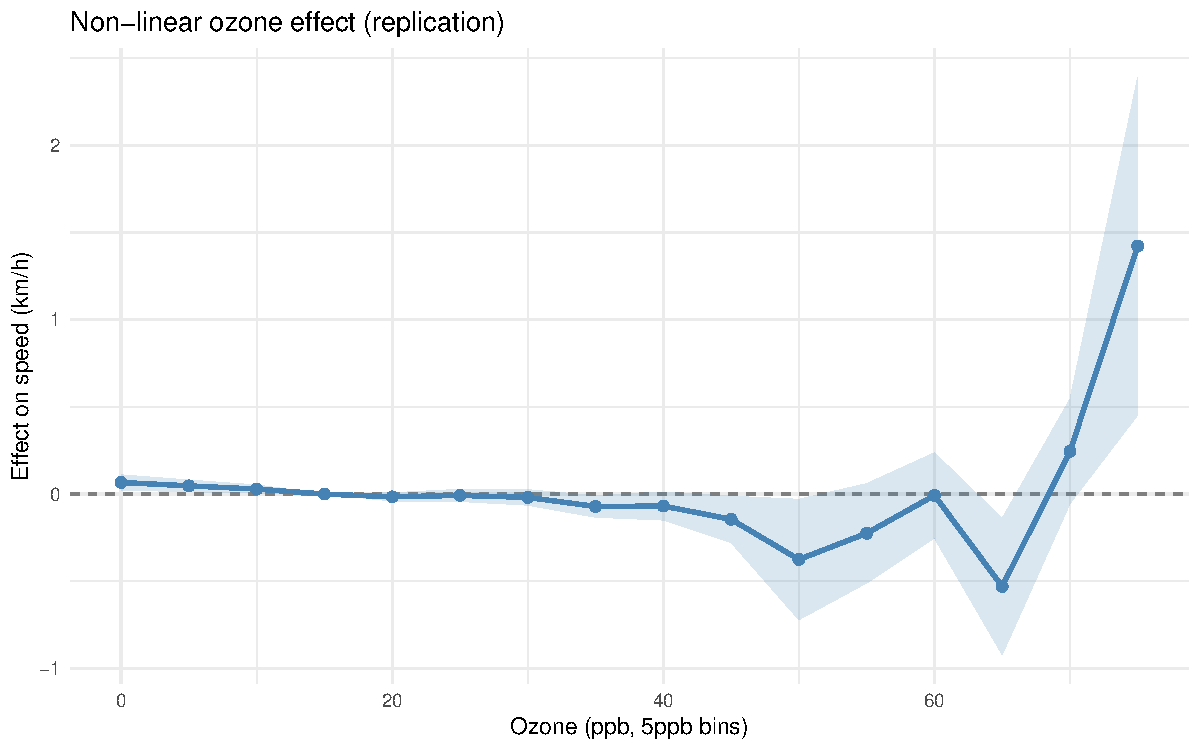
\includegraphics[width=\textwidth]{../output/figures/figure7_replication.pdf}
\caption{2013--2017}
\end{subfigure}
\hfill
\begin{subfigure}[b]{0.32\textwidth}
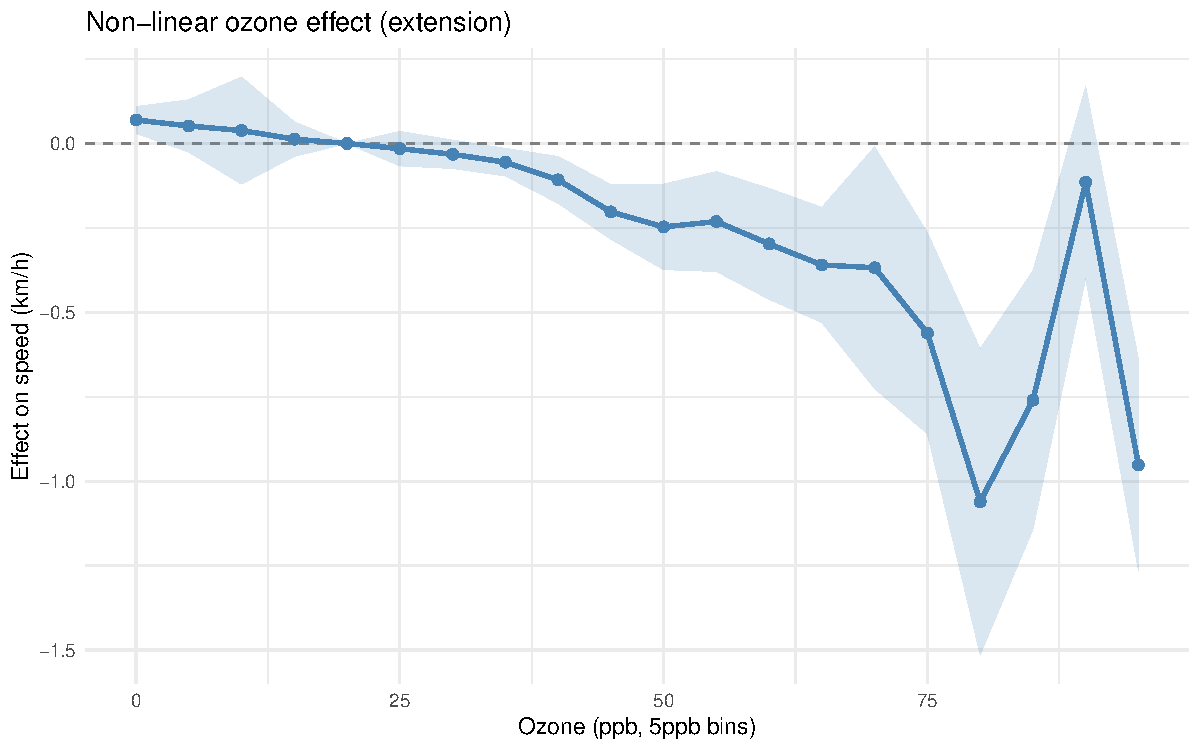
\includegraphics[width=\textwidth]{../output/figures/figure7_extension.pdf}
\caption{2013--2025}
\end{subfigure}
\hfill
\begin{subfigure}[b]{0.32\textwidth}
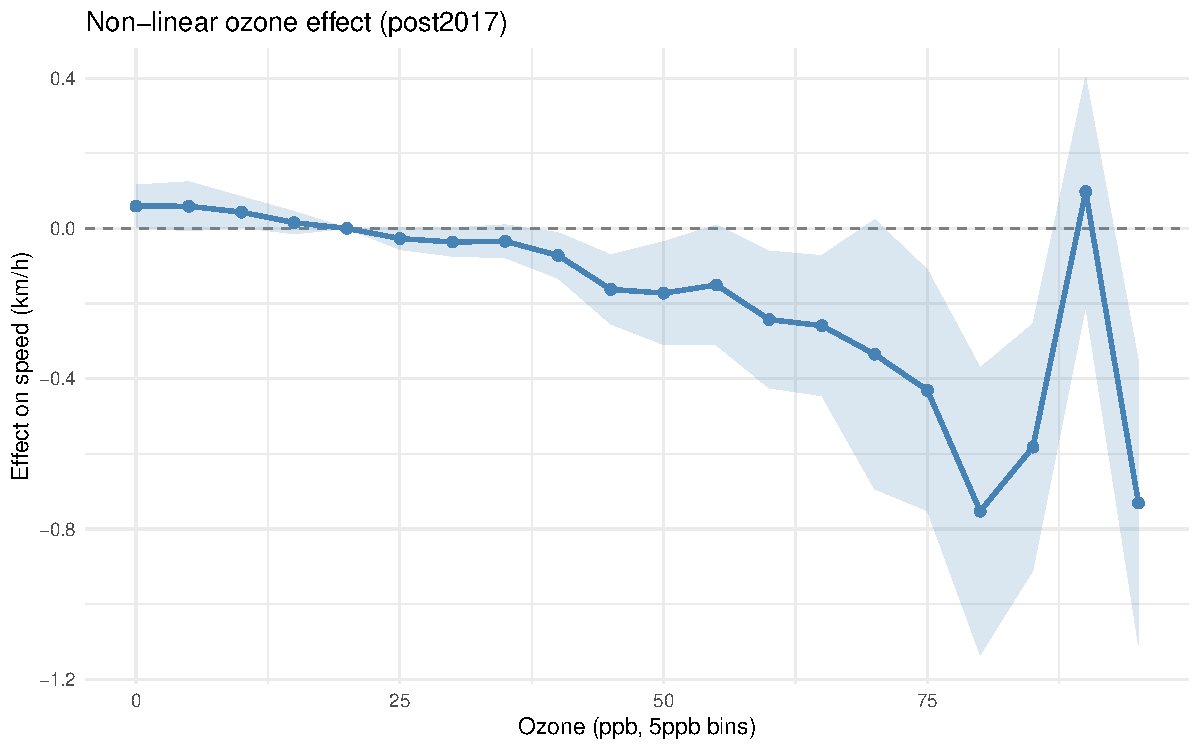
\includegraphics[width=\textwidth]{../output/figures/figure7_post2017.pdf}
\caption{2018--2025}
\end{subfigure}
\caption{Non-linear ozone effects (5~ppb dummies, within-day specification).}
\label{fig:nonlin}
\end{figure}

\paragraph{Lag and lead effects.} Figure~\ref{fig:lagslead} shows the lag/lead analysis. The contemporaneous effect is the strongest, with some persistence in the first lag reflecting ozone autocorrelation. Lead coefficients are near zero, supporting the causal interpretation.

\begin{figure}[H]
\centering
\begin{subfigure}[b]{0.32\textwidth}
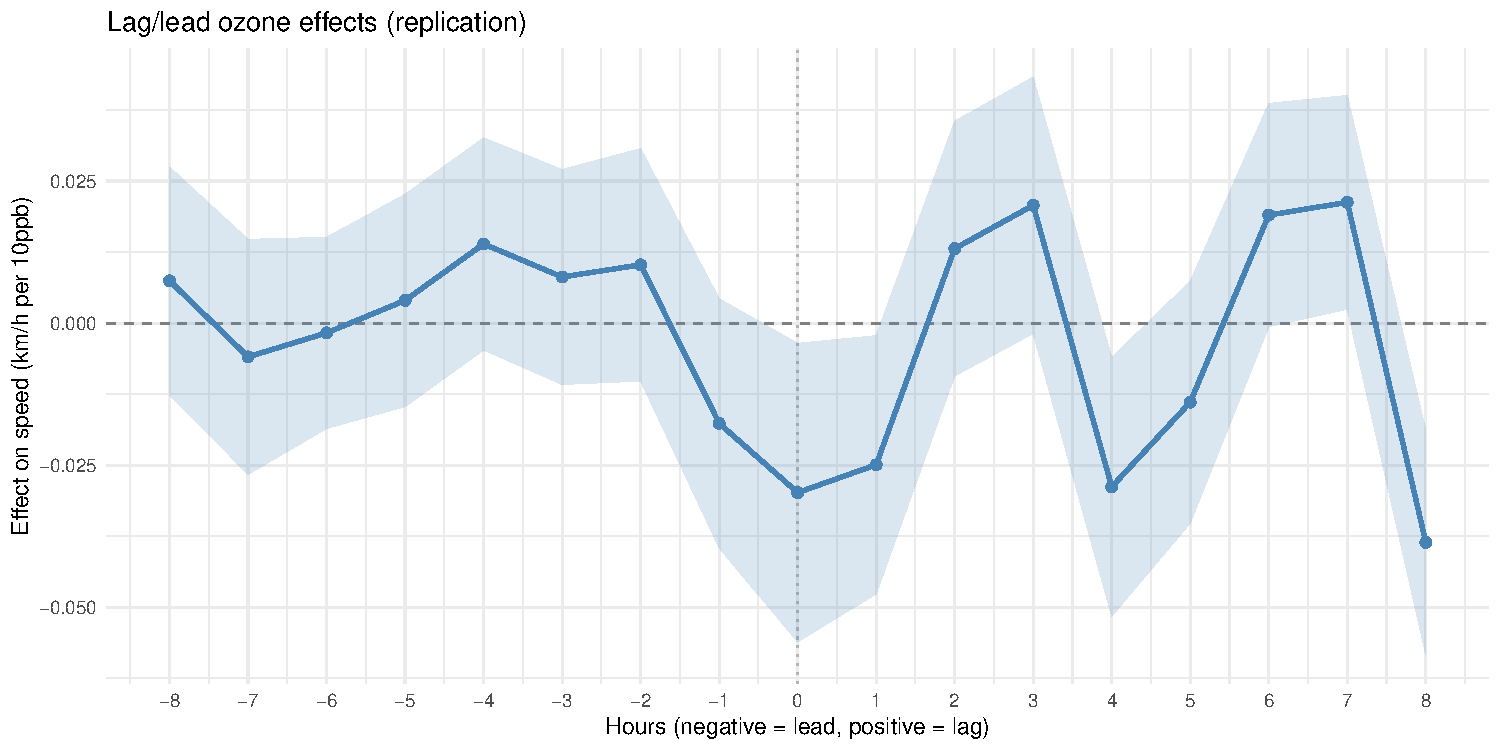
\includegraphics[width=\textwidth]{../output/figures/figure8_replication.pdf}
\caption{2013--2017}
\end{subfigure}
\hfill
\begin{subfigure}[b]{0.32\textwidth}
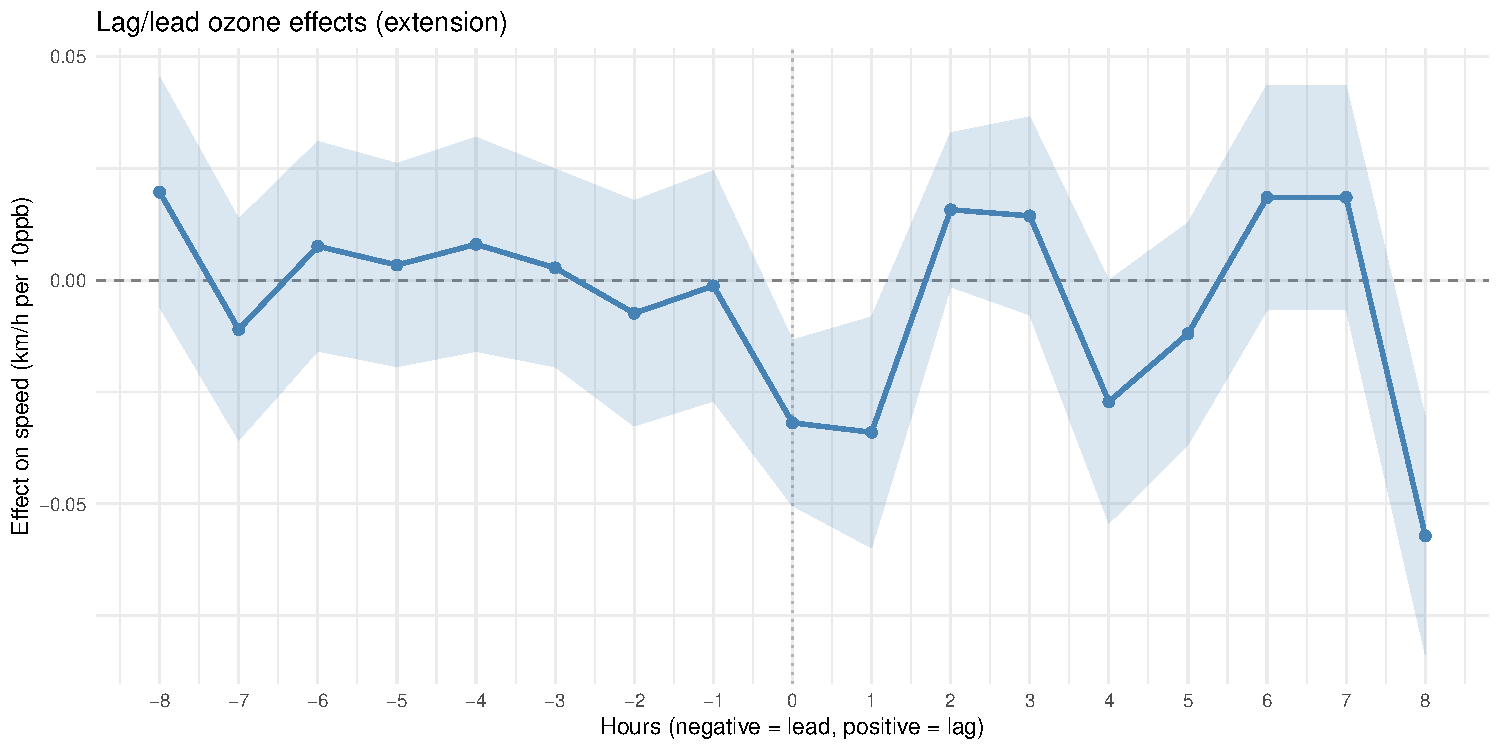
\includegraphics[width=\textwidth]{../output/figures/figure8_extension.pdf}
\caption{2013--2025}
\end{subfigure}
\hfill
\begin{subfigure}[b]{0.32\textwidth}
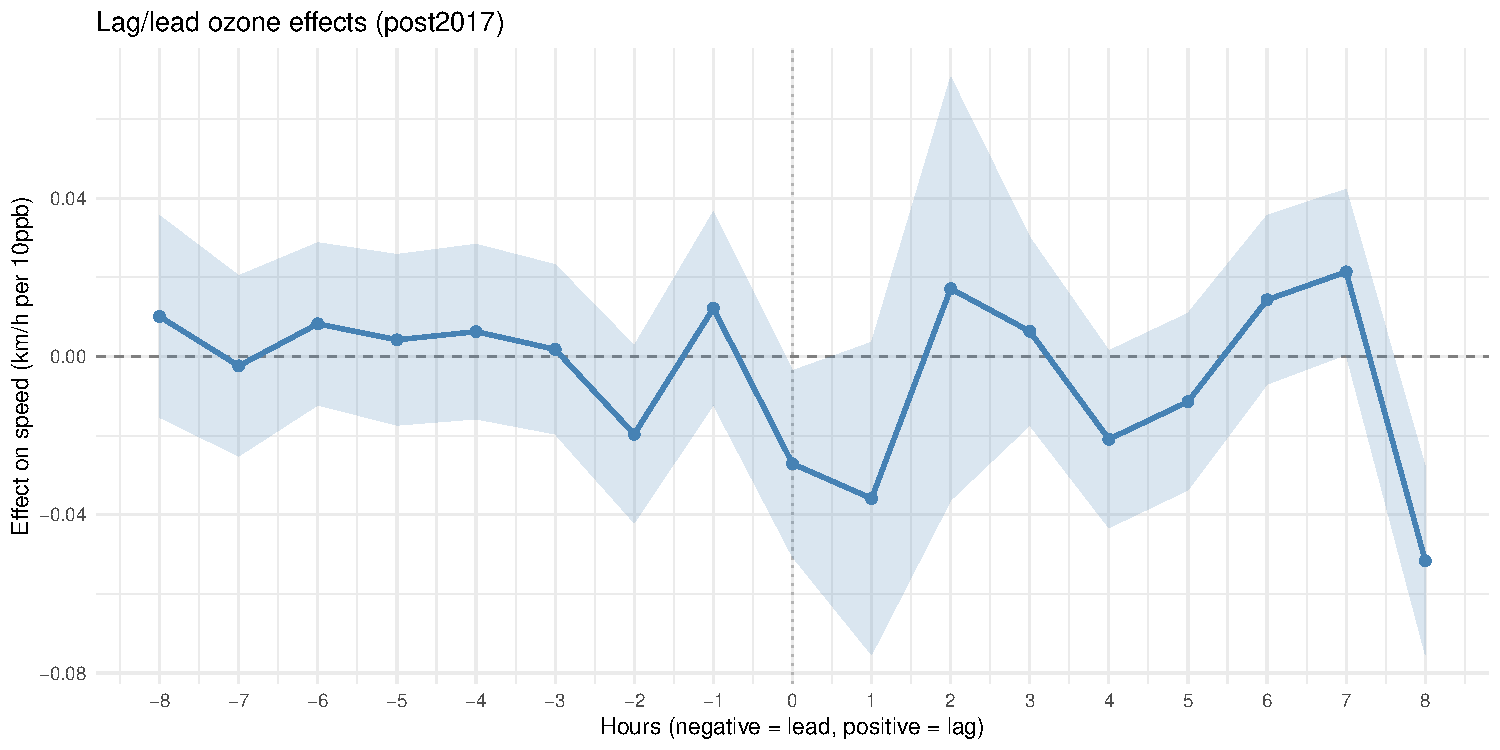
\includegraphics[width=\textwidth]{../output/figures/figure8_post2017.pdf}
\caption{2018--2025}
\end{subfigure}
\caption{Lag and lead ozone effects ($\pm$8 hours, within-day specification).}
\label{fig:lagslead}
\end{figure}

\paragraph{Median speed.} Using median rather than mean speed as the dependent variable yields within-day coefficients of $-0.034$ (replication), $-0.045$ (extension), and $-0.041$ (post-2017), confirming that outliers do not drive the results.


%% ============================================================
\section{Comparison with the Original Study} \label{sec:comparison}
%% ============================================================

Table~\ref{tab:comparison} summarizes the key ozone coefficients from \citet{klingen2020urban} alongside our replication and extension estimates. The coefficient represents the effect of a 10~ppb increase in ozone on cycling speed (km/h).

\begin{table}[H]
\centering
\caption{Comparison of ozone coefficients with \citet{klingen2020urban}.}
\label{tab:comparison}
\begin{tabular}{lcccc}
\toprule
Strategy & Original & Replication & Extension & Post-2017 \\
         & (2013--2017) & (2013--2017) & (2013--2025) & (2018--2025) \\
\midrule
Within-day        & $-0.053^{***}$ & $-0.047^{***}$ & $-0.057^{***}$ & $-0.050^{***}$ \\
Between-day       & $-0.083^{***}$ & $-0.246^{***}$ & $-0.111^{***}$ & $-0.076^{**}$ \\
Spatio-temporal (week) & $-0.044$  & $-0.049$       & $-0.075^{***}$ & $-0.089^{**}$  \\
Panel ($d \geq 0$) & $-0.026$ to $-0.031$ & $-0.014^{***}$ & $-0.009^{***}$ & $-0.007^{**}$ \\
\bottomrule
\end{tabular}

\medskip
\footnotesize Original estimates from \citet{klingen2020urban}: within-day from their Table~2 col.~1; between-day from Table~2 col.~2; spatio-temporal from Table~3 col.~2 (zone-week); panel range from Table~4. Our replication omits traffic controls; the original study showed these to be inconsequential. Our panel confines a pseudo-cyclist to one year-month and excludes electric bikes. $^{***}$, $^{**}$: significant at 1\%, 5\%.
\end{table}

Several patterns emerge from the comparison. First, the within-day replication ($-0.047$) is close to the original ($-0.053$), confirming that omitting traffic controls does not materially affect the estimate, as the original authors demonstrated. Second, the within-day effect is stable over time ($-0.050$ in the post-2017 period), despite higher ozone levels (25.2 vs.\ 18.7~ppb mean). Third, our between-day replication ($-0.246$) exceeds the original ($-0.083$); this difference likely reflects different weather data sources (Open-Meteo vs.\ Met Office) and the absence of traffic controls, to which the between-day specification may be more sensitive. Fourth, the spatio-temporal estimates, while imprecise in the replication period, become significant in the extended and post-2017 samples as statistical power increases. Finally, the panel estimates ($-0.014$ to $-0.007$) are smaller than the original range and decline over time, but remain statistically significant, so ozone also reduces speed within pseudo-cyclists.

%% ============================================================
\section{Conclusion} \label{sec:conclusion}
%% ============================================================

We replicate and extend \citet{klingen2020urban} using 112 million London bike-share trips spanning 2013--2025. The core finding---that ambient ozone reduces cycling speed at concentrations well below regulatory standards---holds in all four identification strategies, although the spatio-temporal estimate is imprecise for 2013--2017. The within-day estimate is stable across periods. The within-cyclist estimate is about half the original one once pseudo-cyclists are confined to one year-month, and is smaller after 2017.

The persistence of this effect through COVID-19, ULEZ expansion, and cycling infrastructure growth---and across a period in which NO$_x$ fell by half while ozone rose by a third---reinforces that it reflects a fundamental physiological response to ozone exposure rather than a statistical artifact of a particular period or pollution mix.

\newpage
\bibliography{references}

\end{document}
